\documentclass{beamer}
\usepackage{graphicx}
\usepackage{verbatim}
\usepackage{alltt}
\usepackage{xcolor}
\usepackage{listings}
\usepackage{hyperref}
\setbeamertemplate{navigation symbols}{}%remove navigation symbols

\renewcommand\UrlFont{\color{blue}}

\newcommand\inputml[1]{\lstinputlisting[language={[Objective]Caml}]{#1}}

\lstdefinelanguage{OCaml}{
  keywords={
    and,as,assert,asr,begin,class,constraint,do,done,downto,effect,else,end,exception,
    external,false,for,fun,function,functor,if,implicit,in,include,inherit,initializer,
    land,lazy,let,lor,lsl,lsr,lxor,macro,match,method,mod,module,mutable,new,object,
    of,open,or,private,rec,sig,struct,then,to,true,try,type,val,virtual,when,
    with,while},
  comment=[s]{(*\ }{\ *)},
}

\definecolor{darkgreen}{rgb}{0,0.2,0}
\definecolor{darkblue}{rgb}{0.1,0.1,0.8}
\definecolor{darkbrown}{rgb}{0.5,0.3,0.0}
\definecolor{grey}{rgb}{0.5,0.5,0.5}
\definecolor{darkgrey}{rgb}{0.2,0.2,0.2}

\lstdefinestyle{ocaml}{
  basicstyle=\ttfamily, % \small
  basewidth=0.5em,
  commentstyle=\color{darkgreen},
  escapeinside={(**}{)},
  keywordstyle=\color{darkblue},
  language=OCaml,
  morekeywords={macro},
  stringstyle=\color{blue},
  showstringspaces=false,
  mathescape=true,
  moredelim=**[is][]{?}{?},
  moredelim=**[is][]{&}{&},
}

\lstdefinestyle{output}{
  basicstyle=\ttfamily\small,
  basewidth=0.5em,
}

\lstset{literate=%
{->}{{$\to$}}2
{...}{{$\ldots$}}2
}

\newcommand\mlkeyword[1]{{\ttfamily\color{darkblue} #1}}

\title[Effects]{Experiences with Effects in OCaml 5.0}
\author[Anil Madhavapeddy and Thomas Leonard]
{Anil Madhavapeddy (speaker) \and Thomas Leonard(speaker) \and Craig Ferguson\and Patrick Ferris\and Sadiq Jaffer\and Tom Kelly \and KC Sivaramakrishnan}
\institute{University of Cambridge and Tarides}
\date[Wasm Stack Switching WG]{WASM Stack Switching WG, Feb 2022}

\begin{document}

\definecolor{grey}{gray}{0.6}

\frame{\titlepage}

% \begin{frame}
% \frametitle{Table of Contents}
% \tableofcontents
% \end{frame}

\begin{frame}
	\frametitle{Overview}
	\begin{itemize}
		\item {Background: OCaml 5.0}
		\item Introduction to effects
		\item Case study: Converting the Angstrom parser
		\item Eio concurrency library
	\end{itemize}
\end{frame}

\begin{frame}[fragile]
	\frametitle{Background: OCaml and the road to 5.0}
	\begin{itemize}
		\item Industrial-grade functional programming language, first released in 1996 and continously developed since then.
    \item Compiles native code binaries for x86/arm/ppc/riscv in 32- and 64-bit.
    \item Also has a portable bytecode compiler that just needs a C compiler, and can
    be compiled to JavaScript (js\_of\_ocaml).
		\item OCaml 5.0 will feature multicore parallelism, and also untyped effects.
		\begin{itemize}
      \item \textbf{Pros:} High-performance direct-style code with a GC (this talk)
      \item \textbf{Cons:} How do retain portability to JavaScript and Wasm?
    \end{itemize}
	\end{itemize}
\end{frame}

\begin{frame}[fragile]
	\frametitle{Background: asynchrony in OCaml 4 and earlier}
	\begin{itemize}
		\item OCaml 4 is single-threaded with no first-class support for concurrency.
    \item IO concurrency has been expressed for years via userlevel libraries that
    allow for futures to be expressed succinctly.
    \item Two widely adopted libraries are:
    \begin{itemize}
      \item Lwt (usually for web programming)
      \item Async (used by Jane Street in their production usage of OCaml)
	  \end{itemize}
  \end{itemize}
\end{frame}


\begin{frame}[fragile]
	\frametitle{OCaml 4.0 Lwt example}
\begin{lstlisting}[style=ocaml]
let foo ~stdin total =
  Lwt_io.read_line stdin >>= fun ->
  Lwt_io.printlf "n/total = %d"
    (int_of_string n / total)
\end{lstlisting}
\begin{lstlisting}[style=output]
Fatal error: exception Division_by_zero
Raised at Lwt_example.foo in file "lwt_example.ml", line 6
Called from Lwt.[...].callback in file "src/core/lwt.ml", ...
\end{lstlisting}
	\begin{itemize}
		\item Backtrace doesn't say what called \verb|foo|
		\item Closure with \verb|total| allocated on the heap
		\item Type of function \verb|foo| appends an \verb|Lwt.t|
	\end{itemize}
\end{frame}

\begin{frame}[fragile]
	\frametitle{OCaml 5.0 effects-based example}
\begin{lstlisting}[style=ocaml]
let foo ~stdin total =
  let n = read_line stdin in
  traceln "n/total = %d"
    (int_of_string n / total)
\end{lstlisting}
\begin{lstlisting}[style=output]
Fatal error: exception Division_by_zero
Raised at Eio_example.foo in file "eio_example.ml", line 11
Called from Eio_example.bar in file "eio_example.ml", line 15
...
\end{lstlisting}
\begin{itemize}
  \item Backtrace is entirely accurate now
  \item Only stack allocation needed for the blocking I/O
  \item Type of function is no longer affected by use of IO
\end{itemize}

\end{frame}

\begin{frame}[fragile]
	\frametitle{Introduction to effects}
	\begin{columns}[t]
		\begin{column}{4.5cm}
	\begin{itemize}
		\item Resumable exceptions
		\item Multiple stacks
	\end{itemize}
		\end{column}
		\begin{column}{5cm}
\begin{lstlisting}[style=ocaml]
effect Foo : int -> int

try
  println "step 1";
  let x = perform (Foo 2) in
  println "step %d" x
with effect (Foo n) k ->
  println "step %d" n;
  continue k (n + 1)
\end{lstlisting}
		\end{column}
	\end{columns}
\end{frame}

\begin{frame}
	\frametitle{Advantages of effects}
	\begin{itemize}
		\item No difference between sequential and concurrent code.
			\begin{itemize}
				\item No special monad syntax.
				\item Can use \mlkeyword{try}, \mlkeyword{match}, \mlkeyword{while}, etc.
				\item No separate lwt or async versions of code.
			\end{itemize}
		\item No heap allocations needed to simulate a stack.
		\item A real stack means backtraces and profiling tools work.
	\end{itemize}
\end{frame}

\begin{frame}
	\frametitle{Case study: Angstrom}

	\url{https://github.com/inhabitedtype/angstrom/}
	\bigskip
	\begin{itemize}
		\item A library for writing parsers
		\item Designed for network protocols
		\item Strong focus on performance
	\end{itemize}
\end{frame}

\begin{frame}[fragile]
	\frametitle{A toy parser}
\begin{lstlisting}[style=ocaml]
type 'a parser = state -> 'a

let any_char state =
  ensure 1 state;
  let c = Input.unsafe_get_char state.input state.pos in
  state.pos <- state.pos + 1;
  c

let (*>) a b state =
  let _ = a state in
  b state
\end{lstlisting}
\end{frame}

\begin{frame}[fragile]
	\frametitle{The Angstrom parser type}
\begin{lstlisting}[style=ocaml,basicstyle=\ttfamily\small]
module State = struct
  type 'a t =
    | Partial of 'a partial
    | Lazy    of 'a t Lazy.t
    | Done    of int * 'a
    | Fail    of int * string list * string
  and 'a partial =
    { committed : int;
      continue  : Bigstringaf.t ->
        off:int -> len:int -> More.t -> 'a t }
end
type 'a with_state = Input.t -> int -> More.t -> 'a
type 'a failure =
  (string list -> string -> 'a State.t) with_state
type ('a, 'r) success = ('a -> 'r State.t) with_state
type 'a parser = { run : 'r.
  ('r failure -> ('a, 'r) success -> 'r State.t) with_state
}
\end{lstlisting}
\end{frame}

\begin{frame}[fragile]
	\frametitle{Angstrom parsers}
\begin{lstlisting}[style=ocaml,basicstyle=\ttfamily\small]
let any_char =
  ensure 1 { run = fun input pos more _fail succ ->
      succ input (pos + 1) more
        (Input.unsafe_get_char input pos)
  }

let (*>) a b =
  { run = fun input pos more fail succ ->
    let succ' input' pos' more' _ =
      b.run input' pos' more' fail succ in
    a.run input pos more fail succ'
  }
\end{lstlisting}
\end{frame}

\begin{frame}[fragile]
	\frametitle{Angstrom : effects branch}
\url{https://github.com/talex5/angstrom/tree/effects}
\bigskip
\begin{lstlisting}[style=ocaml]
type 'a parser = state -> 'a

let any_char state =
  ensure 1 state;
  let c = Input.unsafe_get_char state.input state.pos in
  state.pos <- state.pos + 1;
  c

let (*>) a b state =
  let _ = a state in
  b state
\end{lstlisting}
\end{frame}

\begin{frame}[fragile]
	\frametitle{Parser micro-benchmark}
\begin{lstlisting}[style=ocaml]
let parser = skip_many any_char
\end{lstlisting}
\bigskip
\begin{table}
\begin{tabular}{l|rrrrr}
          & Time     & MinWrds &  MajWrds \\
\hline
Callbacks  & 750.63ms & 160.04Mw & 8,9944.00kw \\
\uncover<2>{Callbacks'} & \uncover<2>{180.73ms} & \uncover<2>{220.01Mw} &   \uncover<2>{9,659.00w} \\
Effects    &  57.81ms &        - &          -
\end{tabular}
\end{table}
\bigskip
\uncover<1>{1}3 times faster!
\pause
\end{frame}

\begin{frame}[fragile]
	\frametitle{Realistic parser benchmark}
Parsing an HTTP request shows smaller gains:
\bigskip
\begin{table}
\begin{tabular}{l|rrrrr}
          & Time     & MinWrds &  MajWrds \\
\hline
Callbacks  &  60.30ms &  9.28Mw & 102.08kw \\
Effects    &  50.71ms &  2.13Mw &  606.30w
\end{tabular}
\end{table}
\end{frame}

\begin{frame}[fragile]
	\frametitle{Using effects for backwards compatibility}
\begin{lstlisting}[style=ocaml]
effect Read : int -> state
let read c = perform (Read c)

let parse p =
  let buffering = Buffering.create () in
  try Unbuffered.parse ~read p
  with effect (Read committed) k ->
    Buffering.shift buffering committed;
    Partial (fun input ->
      Buffering.feed_input buffering input;
      continue k (Buffering.for_reading buffering)
    )
\end{lstlisting}
(simplified)
\end{frame}

\begin{frame}
	\frametitle{Angstrom summary}
	\begin{itemize}
		\item Slightly faster
		\item Much simpler code
		\item No effects in interface
		\item Can convert between callbacks and effects easily
	\end{itemize}
\end{frame}

\begin{frame}
	\frametitle{Eio : an IO library using effects for concurrency}
	\begin{itemize}
		\item Alternative to Lwt and Async
		\item Generic API that performs effects
		\item Cross-platform libuv effect handler
		\item High-performance io-uring handler for Linux
	\end{itemize}
\end{frame}

\begin{frame}[fragile]
	\frametitle{Eio example}
\begin{lstlisting}[style=ocaml]
let handle_connection =
  Httpaf_eio.Server.create_connection_handler
    ~config
    ~request_handler
    ~error_handler

let main ~net =
  Switch.top @@ fun sw ->
  let socket = Eio.Net.listen ~sw net (`Tcp (host, port))
    ~reuse_addr:true
    ~backlog:1000 
  in
  while true do
    Eio.Net.accept_sub ~sw socket handle_connection
      ~on_error:log_connection_error 
  done
\end{lstlisting}
\end{frame}

\begin{frame}
	\frametitle{HTTP benchmark}
	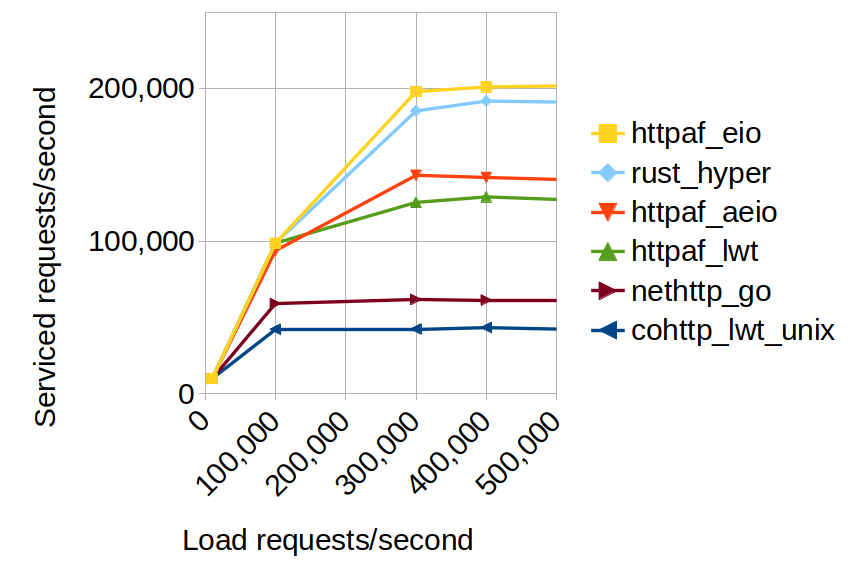
\includegraphics[width=\textwidth]{rps-graph.png}
	100 concurrent connections. Servers limited to 1 core.
\end{frame}

\begin{frame}
	\frametitle{Eio : other features}
	\begin{itemize}
		\item Structured concurrency
		\item OCaps security model
		\item Tracing support
		\item Supports multiple cores
		\item Still experimental
	\end{itemize}
	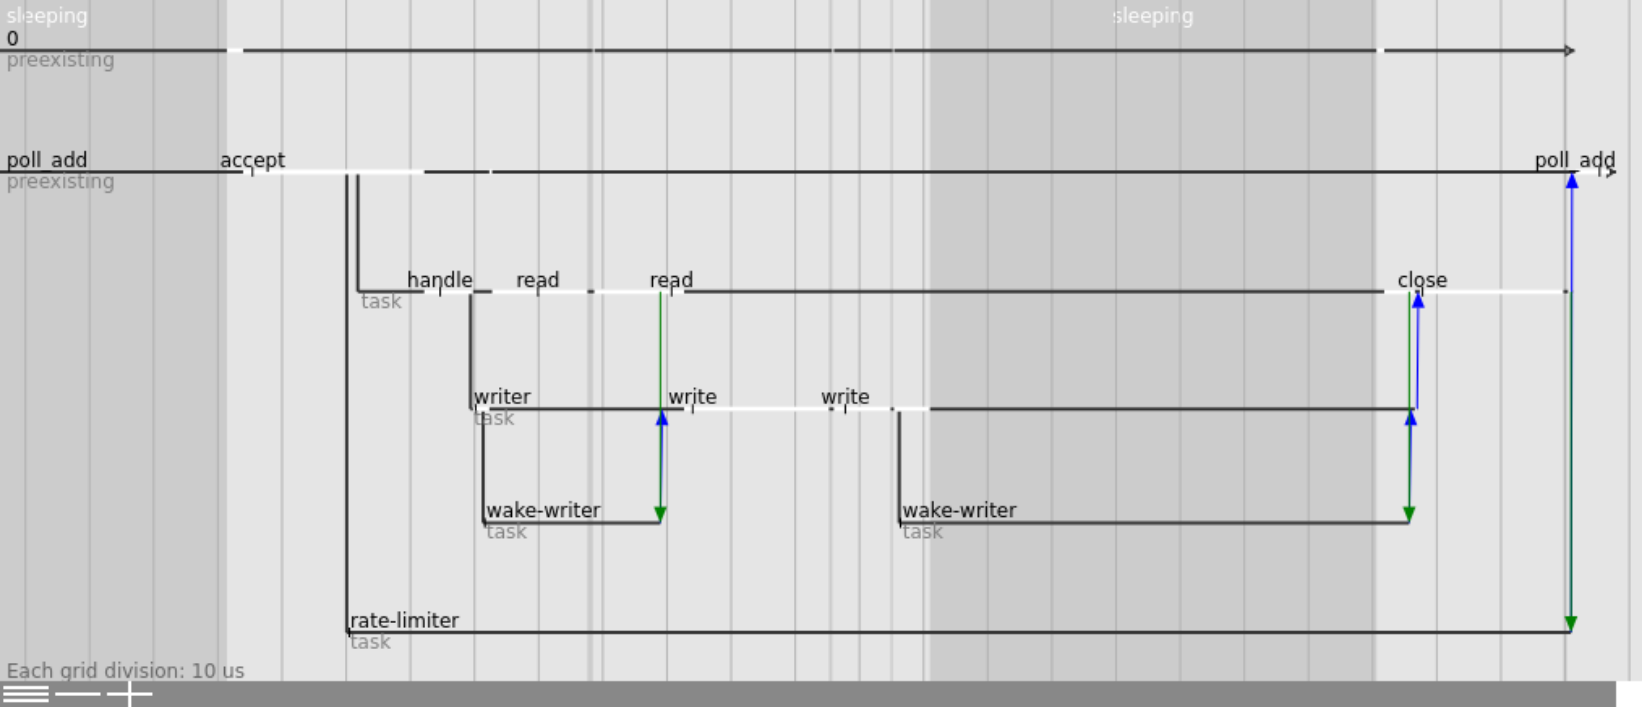
\includegraphics[width=\textwidth]{trace.png}
\end{frame}

\begin{frame}
	\frametitle{Summary of OCaml 5.0 and our use of effects}
	\begin{itemize}
		\item Concurrency with effects works very well and is ergonomic to program with
		\item Effects have very good performance (stack vs heap)
		\item The use of separate of effect schedulers is still emerging, but there are dozens
		of networking/storage OCaml libraries being ported currently, with little drama.
    \item Key open blocker for our community is Js/Wasm compilation support:
    \textbf{effects are here to stay in OCaml 5.0, so what's the best path forward?}
	\end{itemize}
	\bigskip
	\url{https://github.com/ocaml-multicore/eio} documentation shows how to try out OCaml effects.
  \url{https://github.com/patricoferris/awesome-multicore-ocaml} lists community libraries.
\end{frame}

% Backup slides



\end{document}
